\documentclass[letterpaper]{article}
\usepackage{underscore}
\usepackage[left=2.0cm, right=2.0cm, top=1.0cm]{geometry}
\usepackage[utf8]{inputenc}
\usepackage{graphicx}
\usepackage{graphics}
\usepackage[spanish]{babel}
\usepackage{lipsum}
\usepackage{float}
\usepackage{subfigure}
\usepackage{csquotes}
\usepackage{color}
\usepackage{colortbl}
\usepackage{xcolor}

\title{EV\_2\_8\_calcular\_los\_parametros\_de\_circuitos\_de\_activación\_de\_transistores\_de\_potencia}
\author{Ledesma Hernández Miguel Ángel}
\date{28/October/2019}

\begin{document}
\begin{figure}[t]
    
\includegraphics[width=6cm]{img/logo.png}
\end{figure}
\vspace{2cm}
\maketitle
\vspace{12cm}
\begin{center}
   Universidad politécnica de la zona metropolitana de Guadalajara.\\
Sistemas electrónicos de interfaz.\\
4-A Mecatrónica.\\ 
\end{center}
\newpage
Un transistor tiene la capasidad de ser analógico o digital; es decir, el analógico funciona como amplificador de onda, y el dígital se utiliza como un switch, para información de ceros y unos en todo caso si queremos trabajar como amplificador se debe utilizar la polarización. Pero este al no ser el caso queremos usar como digital, es decir; corte y saturación.\\
Como queremos usarla de manera digital debemos entender ¿cómo funciona un transistor?, para poder calcular su activación.\\
un transistor pnp tiene una tensión, base, emisor, esta tensión dependiendo el material del transistor[germanio: 0.3 y silicio 0.7] si no es superada es decir : $V_{BE} < 0.7V$ entonces tendremos un "switch cerrado", pero si encontramos que es mayor ó mucho mayor, es decir: $V_{BE}>0.7V  ||  V_{BE}>>0.7V$ entonces se comportará como un switch cerrado y por tanto podremos ver que la corriente del emisor es igual que la corriente del colector, mientras que en el estado 0, $V_{BE} < 0.7V $ encontraremos que la corriente es = 0 en la base y el colector,sin embargo encontramos que la corriente en la base es mayor a cero. Así podemos ver en palabras simples "un paso o no paso".\\
Para lograr esto debemos calcular la resistencia de la base, esta se obtiene de calcular la siguiente fórmula:\\

\begin{figure}[htbp]
\centering
\begin{huge}
	$R_{base}=\frac{(V_{in}-V_{trans})*hFe}{I_{colector}}$\\
\end{huge}
\end{figure}
	


\begin{large}
	\textbf{Significado cada variable}\\
\end{large}
	\begin{itemize}
		\item $R_{base}$ : La resistencia de la base es la que se necesita en la pata base como lo dice su nombre para poder activar el transistor.
		\item $V_{in}$ : Este es el voltaje que entrará a la base del transistor. 
		\item $V_trans$ : Este número es una constante, dependiendo del material de nuestro transistor; por ejemplo si nuestro transistor es de 
		\begin{itemize}
		\item Germanio será un voltaje de activación de 0.3V
		\item Silicio será un voltaje de activación de 0.6V
		\end{itemize}
		\item $hFe$ : Es la ganancia de corriente que tiene el transistor, este se obtiene cuando mides en la opción de "hFe", en el multímetro, introduciendo según sea nuestro transistor y el acomodo de sus patas y si es npn o pnp, dependiendo tambien de su datasheet.
		\item $I_{colector}$ : Ésta es la intesidad que tiene el colector en el momento de activación, para obtenerlo se usa ley de Ohm, con la formula de $I_c= \frac{V_{cc}}{R_{cc}}$
	\end{itemize}

\begin{large}
\textbf{Cómo resolver:}
\end{large}
\begin{itemize}
	\item Se sustituyen los valores por los que se piden\\
	$R_{base}=\frac{(5V-0.7)*75}{4mA}$\\
	\item Como en casi todas las operaciones se reducen terminos, para simplificar.\\
	$R_{base}=\frac{(4.3)*75}{4mA}$
	\item Multiplicamos $ (V_{in}-V_{trans})*hFe $\\ 
	$R_{base}=\frac{322.5}{4mA}$
	\item Dividimos normalmente\\
	$R_{base} = 806.25\Omega $
\end{itemize}
\newpage
\begin{figure}[hbtp]
\caption{identificación de partes}
\centering
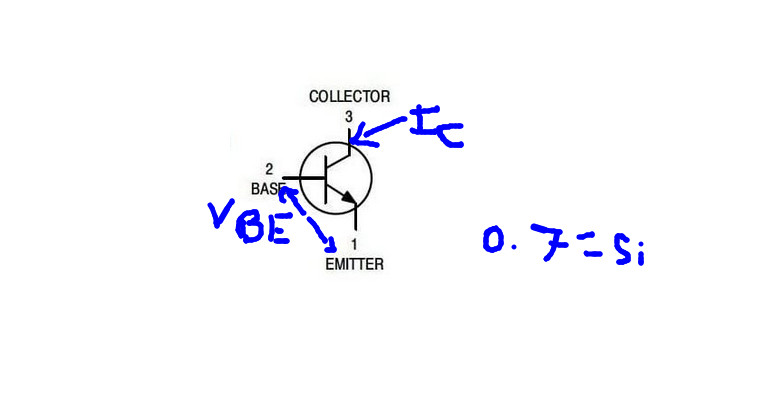
\includegraphics[scale=0.5]{img/dadada.jpg}
\end{figure}

\end{document}
